\documentclass[a4paper,12pt]{article}

\usepackage[utf8x]{inputenc}
\usepackage[english]{babel}
\usepackage[margin=1in,includefoot]{geometry}

\usepackage{pgfplots}
\pgfplotsset{width=11cm,compat=1.12}
\usetikzlibrary{arrows}
\usepackage{amsmath}

\usepackage{indentfirst}
\usepackage{booktabs}

\usepackage[backref=false,pagebackref=true,citecolor=blue]{hyperref}
\hypersetup{colorlinks=true,urlcolor=blue,pdfborder={0 0 0}}

\setlength{\parindent}{2em}
\setlength{\parskip}{1em}

%\renewcommand{\arraystretch}{2}
%\renewcommand{\familydefault}{\sfdefault}

\usepackage{minted}
\renewcommand{\theFancyVerbLine}{\rmfamily\scriptsize\arabic{FancyVerbLine}}
\definecolor{whitesmoke}{rgb}{0.96,0.96,0.96}
\setminted{linenos,autogobble,breaklines,fontsize=\footnotesize,tabsize=4,numbersep=7pt,bgcolor=whitesmoke}
% \begin{minted}{cpp}
% \mintinline{cpp}{...}

\newcommand{\refspace}{\vspace{-2mm}}
\newcommand{\redarrow}{\textcolor{blue}{$\mathbf{\Rightarrow}$}}
\makeatletter
\def\BR@@bibitem#1#2\par{
	\let\backrefprint\BR@backrefprint
	\def\@linkcolor{black}
	\BRorg@bibitem{#1}#2\redarrow \thinspace \BR@backref{#1}
}
\makeatother

\author{Roland Bogosi}
\title{Market Prediction}

\begin{document}
\thispagestyle{empty}
	 
	\begin{center}
		\vspace{3.1in}
		
		{\sffamily\huge Market Prediction using Neural Networks}
		
		\vspace{0.4in}
		
		{\sffamily\LARGE Assignment Report}
		
		\vspace{0.3in}
		
		{\sffamily\Large January 4th, 2016}
		
		\vspace{3.2in}
	\end{center}
	
	\begin{flushright}
		{\sffamily\itshape\Large Roland Bogosi}
	\end{flushright}

\newpage
\thispagestyle{empty}
\section*{Table of Contents}

	\begingroup
	\renewcommand{\section}[2]{}
	\hypersetup{linkcolor=blue}
	\setlength{\parskip}{0em}
	\tableofcontents
	\endgroup

\newpage
\section{Introduction} \label{intro}

	The purpose of this classroom assignment is to use neural networks in order to predict stock market or currency fluctuations. There are many ways to tackle this time-series prediction problem, each of them having their own pros and cons:
	
	\textbf{Index Prediction} -- Try to teach the individual values of a series. This way the neural network will receive an input which in some form indicates the day we would like to evaluate it/predict for and as the output of the network, we get the prediction.
	
	\textbf{Indicator Prediction} -- Transform the dataset into indicators used during stock analysis, and teach the neural network the pattern of these. This way, the neural network will not be able to predict the index itself, but it should be able to predict the trend within the indicator that is used to make the actual decision if a stock should be purchased or not.
		
	In both cases, as described in \cite{op1997stock}, one of the main challenges was to decide what inputs and outputs should the neural network be trained for. My initial thought was to feed the date as input, and get the predicted index as the output. However, upon experimentation I learned that this model would not work, and after further researching, the winner method seemed to be having one or more input variables which are the index values of the previous days.

	\begin{figure}[!htbp]
		\centering
		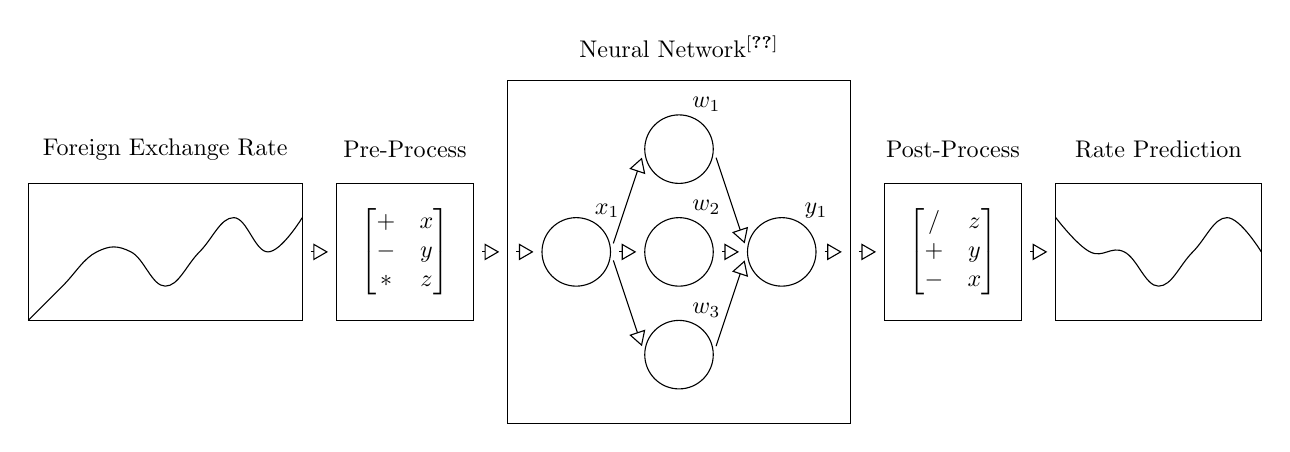
\begin{tikzpicture}[scale=0.87, transform shape]
		\tikzstyle{es} = [-open triangle 60]
		\draw [] (0,0) ellipse (0.5 and 0.5);
		\draw [] (0,1.5) ellipse (0.5 and 0.5);
		\draw [] (0,-1.5) ellipse (0.5 and 0.5);
		\draw [] (1.5,0) ellipse (0.5 and 0.5);
		\draw [] (-1.5,0) ellipse (0.5 and 0.5);
		\node (v1) at (-1,0) {};
		\node (v2) at (-0.5,1.5) {};
		\node (v3) at (-0.5,0) {};
		\node (v4) at (-0.5,-1.5) {};
		\node (v5) at (0.5,1.5) {};
		\node (v7) at (0.5,0) {};
		\node (v8) at (0.5,-1.5) {};
		\node (v6) at (1,0) {};
		\draw [es] (v1) edge (v2);
		\draw [es] (v1) edge (v3);
		\draw [es] (v1) edge (v4);
		\draw [es] (v5) edge (v6);
		\draw [es] (v7) edge (v6);
		\draw [es] (v8) edge (v6);
		\node (v9) at (-2.5,0) {};
		\node (v12) at (2.5,0) {};
		\node (v10) at (-2,0) {};
		\draw [es] (v9) edge (v10);
		\node (v11) at (2,0) {};
		\draw [es] (v11) edge (v12);
		\node at (0.4,2.15) {$w_1$};
		\node at (0.4,0.65) {$w_2$};
		\node at (0.4,-0.85) {$w_3$};
		\node at (2,0.6) {$y_1$};
		\node at (-1.05,0.6) {$x_1$};
		\node at (0,3) {Neural Network$^{[\ref{neurnet}]}$};
		\draw  (-2.5,2.5) rectangle (2.5,-2.5);
		\draw  (-5.5,-1) rectangle (-9.5,1);
		\draw  plot[smooth, tension=.7] coordinates {(-9.5,-1) (-9,-0.5) (-8.5,0) (-8,0) (-7.5,-0.5) (-7,0) (-6.5,0.5) (-6,0) (-5.5,0.5)};
		\node at (-7.5,1.5) {Foreign Exchange Rate};
		\node (v13) at (-5.5,0) {};
		\node at (-4,1.5) {Pre-Process};
		\draw [es] (-5,1) rectangle (-3,-1);
		\node (v14) at (-5,0) {};
		\node (v15) at (-3,0) {};
		\draw [es] (v13) edge (v14);
		\draw [es] (v15) edge (v9);
		\draw [es] (3,1) rectangle (5,-1);
		\node (v16) at (3,0) {};
		\node (v17) at (5,0) {};
		\node at (4,1.5) {Post-Process};
		\draw [es] (v12) edge (v16);
		\draw  (8.5,-1) rectangle (5.5,1);
		\draw  plot[smooth, tension=.7] coordinates {(5.5,0.5) (6,0) (6.5,0) (7,-0.5) (7.5,0) (8,0.5) (8.5,0)};
		\node at (7,1.5) {Rate Prediction};
		\node (v18) at (5.5,0) {};
		\draw [es] (v17) edge (v18);
		\node at (-4,0) {$ \begin{bmatrix}+ & x\\ - & y\\ * & z\end{bmatrix} $};
		\node at (4,0) {$ \begin{bmatrix}/ & z\\ + & y\\ - & x\end{bmatrix} $};
		\end{tikzpicture}
		\caption{Basic Architecture of the System}
		\label{sysarch}
	\end{figure}
	
	For the purposes of this classroom assignment, I decided focusing on using currency rates, since stock data has way too many outside factors influencing it. I would have had to analyze these outside factors for each stock individually and encode it as an input to the neural network in some form, in order to create an accurate model. For example, the stock of a car manufacturing company might go up when they hold a press release and announce a model, and might suddenly go down if the new model gets a bad review from a reputable source or an issue arises with it, possibly needing call-backs.

\newpage
\section{Network Structure}

	After examining existing papers in the field of stocks and neural networks, I came upon paper \cite{guresen2011using} which summarizes a multitude of previous experiments done in this topic, including the neural networks and training sets used with the varying degrees of success.

	\begin{figure}[!htbp]
		\centering
		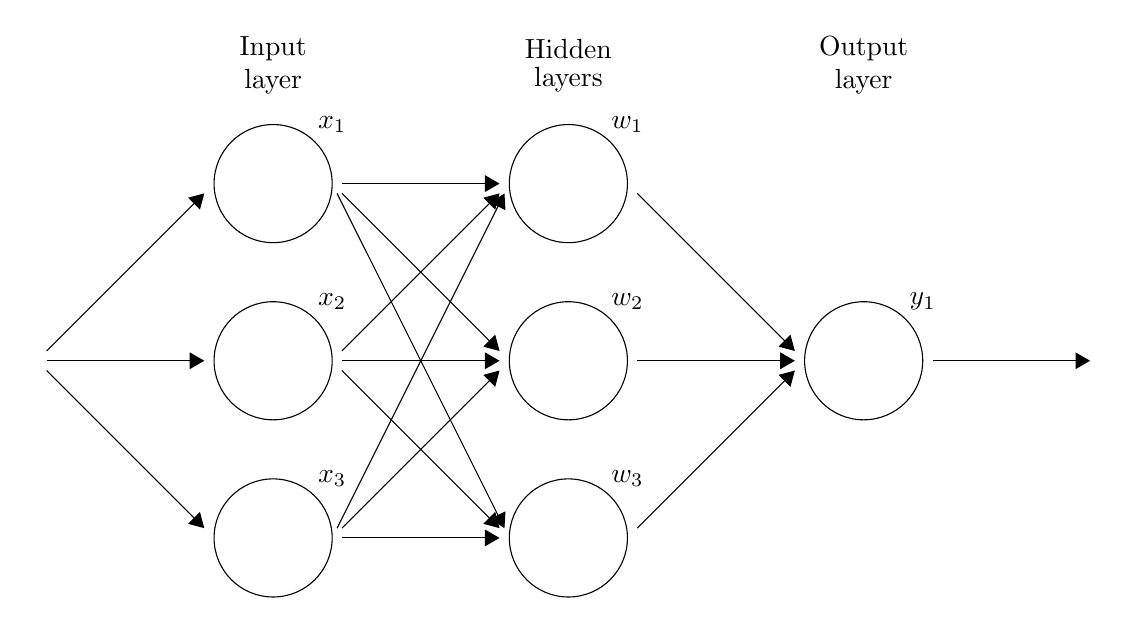
\begin{tikzpicture}[x=1.5cm,y=1.5cm]
			\tikzstyle{es} = [-triangle 60]
			\draw [] (0,0) ellipse (0.5 and 0.5);
			\draw [] (0,1.5) ellipse (0.5 and 0.5);
			\draw [] (0,-1.5) ellipse (0.5 and 0.5);
			\draw [] (2.5,0) ellipse (0.5 and 0.5);
			\draw [] (-2.5,0) ellipse (0.5 and 0.5);
			\node (v1) at (-2,0) {};
			\node (v2) at (-0.5,1.5) {};
			\node (v3) at (-0.5,0) {};
			\node (v4) at (-0.5,-1.5) {};
			\node (v5) at (0.5,1.5) {};
			\node (v7) at (0.5,0) {};
			\node (v8) at (0.5,-1.5) {};
			\node (v6) at (2,0) {};
			\draw [es] (v1) edge (v2);
			\draw [es] (v1) edge (v3);
			\draw [es] (v1) edge (v4);
			\draw [es] (v5) edge (v6);
			\draw [es] (v7) edge (v6);
			\draw [es] (v8) edge (v6);
			\node (v9) at (-4.5,0) {};
			\node (v12) at (4.5,0) {};
			\node (v10) at (-3,0) {};
			\draw [es] (v9) edge (v10);
			\node (v11) at (3,0) {};
			\draw [es] (v11) edge (v12);
			\node at (-2.5,2.5) {\shortstack{Input\\layer}};
			\node at (0,2.5) {\shortstack{Hidden\\layers}};
			\node at (2.5,2.5) {\shortstack{Output\\layer}};
			\node at (0.5,2) {$w_1$};
			\node at (0.5,0.5) {$w_2$};
			\node at (0.5,-1) {$w_3$};
			\node at (3,0.5) {$y_1$};
			\node at (-2,0.5) {$x_2$};
			\draw  (-2.5,1.5) ellipse (0.5 and 0.5);
			\draw  (-2.5,-1.5) ellipse (0.5 and 0.5);
			\node (v13) at (-3,1.5) {};
			\node (v15) at (-2,1.5) {};
			\node (v14) at (-3,-1.5) {};
			\node (v16) at (-2,-1.5) {};
			\node at (-2,2) {$x_1$};
			\node at (-2,-1) {$x_3$};
			\draw [es] (v9) edge (v13);
			\draw [es] (v9) edge (v14);
			\draw [es] (v15) edge (v2);
			\draw [es] (v15) edge (v3);
			\draw [es] (v15) edge (v4);
			\draw [es] (v16) edge (v4);
			\draw [es] (v16) edge (v3);
			\draw [es] (v16) edge (v2);
		\end{tikzpicture}
		\caption{Structure of the Neural Network}
		\label{neurnet}
	\end{figure}

	The neural network shown in figure \ref{neurnet} is a multilayer perceptron network, whose purpose generally is to map a set of inputs onto a set of outputs, as such its application is popular for solving time-series prediction problems. It has a variable number of inputs, $x_1$ through $x_n$, which are the indices of the stock or currency for those days. The output of the network, $y_1$, is the predicted value for the \textit{next} day.
	
	The number of hidden layers in the network varies based on how many training samples (days) we would like to train the network on, and also on how many days we would like to predict beyond the training samples. While the general rule is to have $x_n \cdot 2$ hidden layers, I evaluated this during several trial and error runs and it did not seem to work well with this application. Even with the momentum learning parameter ($m$) set to a high value, $0.9 < m < 1$, the neural network was not able to accurately fit the data, it only generated an approximate oscillation.
	
	The neural network is trained with backpropagation, which is a supervised learning method. The network weights are randomly initialized to values between the range of $[0.25..0.35]$, which was determined to yield the best results after a few trial and error runs. The activation function used with the trainer is sigmoid: $f(x) = \frac{1}{e^{-\alpha \cdot x} + 1}$
	
	After some experimentation, I found the number of hidden layers in order to accurately fit the data as a result of $1,000$ iterations of the backpropagation teacher algorithm, to be an approximation of the size of training samples. As such, the network configuration will vary for each experiment individually.

\section{Usage Intricacies}
\subsection{Error Calculation} \label{mape}

	As shown later on, I conducted a multitude of experiments in order to try and find a configuration with the lowest learning and prediction error for each common training size and prediction requirement. However, in order to quantify the error, I had to look up the methods available for determining the accuracy of trend estimation and found a comparison between the common methods in paper \cite{armstrong1992error}.
	
	\textit{MAPE} (\textit{Mean Absolute Percentage Error}) ended up as being the winning method, since it has been used in many other papers, such as \cite{majhi2009efficient}, which allows me to have a baseline comparison for my results. \textit{MAPE} is defined as:\\
	$$ \epsilon = (\frac{1}{n} \sum_{i=1}^{n} \frac{| x_i - x_i' |}{x_i}) \cdot 100 $$\\
	where $n$ is the number of predictions, $x_i$ is the actual value, and $x_i'$ is the predicted value.
	
\subsection{Parameter Optimization} \label{paramopt}
	
	In order to find the best possible parameters for any given dataset and any requested prediction size, I set up a script to find the most optimal parameters for the given dataset by training and evaluating neural networks with varying parameters using the \mintinline{csharp}{MarketPrediction.NeuralNetwork.TrainAndEval()} API. A snippet of this script can be observed in listing \ref{bruteforce}.
	
	\begin{listing}[!htbp]
		\begin{minted}{csharp}
double smallestError = double.MaxValue;

for (int inputLayers = 1; inputLayers < min(10, dataSetSize); inputLayers++) {
	for (int hiddenLayers = 1; hiddenLayers < dataSetSize; hiddenLayers++) {
		// ...additional parameters as needed...
		
		double error = TrainAndEval(inputLayers, hiddenLayers, ...);
		
		if (error < smallestError) {
			// save current parameters as best-performing...
			smallestError = error;
		}
	}
}
		\end{minted}
		\caption{Exhaustive Search for Highest Accuracy}
		\label{bruteforce}
	\end{listing}
	
\newpage
	The complexity of finding the most optimal parameters for any given input is:\\
	$$ \mathcal{O}(\prod_{i=1}^{P_n} \sum_{j=1}^{P_{i,m}} P_{i,j}) $$\\
	where $P_n$ is the number of parameters being optimized for, $P_{i,m}$ is the number of possible options within that parameter, and $P_{i,j}$ is the number of neural networks that need to be trained in order to determine the error accurately. This number is usually $1$, however for parameters where there are random factors, this number can be higher, and then the error can be the average of all runs with that parameter.
	
	Since this optimization problem is composed of a multitude of independent loops, it can easily be parallelized by asynchronously running one or more of the loops. As such, it becomes a fast and easy method to find the best configuration for any data set. The error value the search is optimizing for is the \textit{MAPE} value, as described in section \ref{mape}.
	
\section{Experiments}
\subsection{7-day Prediction for any 30-day EUR/USD Data} \label{pred730nn}
	
	In this experiment, I focused my efforts on tuning a neural network to predict as accurately as possible a full week's exchange rates in advance for the currency pair EUR/USD.
	
	\begin{figure}[!htbp]
		\centering
		\begin{tikzpicture}
		\begin{axis}[
			xlabel={Days},
			ylabel={Index},
			legend pos=north west,
			ymajorgrids=true,
			grid style=dashed,
			every axis plot/.append style={line width=1pt},
			legend entries={Actual Rates,Estimate,Prediction}
		]
			\addplot[blue,smooth]  table {eur_usd_august_30.txt};
			\addplot[red,smooth]   table {eur_usd_august_30_neuron.txt};
			\addplot[green,smooth] table {eur_usd_august_30_neuron_pred.txt};
		\end{axis}
		\end{tikzpicture}
		\caption{EUR/USD Rates for August 2015 using Neural Networks}
		\label{eur_usd_august_30_neuron}
	\end{figure}
	
	The network shown in figure \ref{eur_usd_august_30_neuron} was trained for $1,000$ iterations, with a \textit{learning rate} of $0.05$ and a \textit{momentum learning coefficient} of $0$. It has $3$ inputs and $8$ hidden layers.
	
	Its mean absolute percentage error for the training set is $0.4825\%$, while the prediction error for the next 7 days is $0.2790\%$.
	
	\begin{figure}[!htbp]
		\centering
		\begin{tikzpicture}
		\begin{axis}[
			xlabel={Days},
			ylabel={Index},
			legend pos=north west,
			ymajorgrids=true,
			grid style=dashed,
			every axis plot/.append style={line width=1pt},
			legend entries={Actual Rates,Estimate,Prediction}
		]
			\addplot[blue,smooth]  table {eur_usd_august_30.txt};
			\addplot[red,smooth]   table {eur_usd_august_30_genetic.txt};
			\addplot[green,smooth] table {eur_usd_august_30_genetic_pred.txt};
		\end{axis}
		\end{tikzpicture}
		\caption{EUR/USD Rates for August 2015 using Genetic Algorithms}
		\label{eur_usd_august_30_genetic}
	\end{figure}
	
	As a comparison, in figure \ref{eur_usd_august_30_genetic}, the same dataset is taught with a genetic algorithm. The algorithm ran for $10,000$ iterations, while having a population size of $100$ and using a selection method which selects the chromosomes with the highest fitness value. The configuration had 10 variable inputs and 3 constants, as explained in table \ref{geninput}.

	\begin{table}[!htbp]
		\centering
		\begin{tabular}{@{}lclr@{}}
			\toprule
			\textbf{\$} & \textbf{Value} & \multicolumn{1}{c}{\textbf{Explanation}} & \textbf{Type} \\ \midrule
			a..j & $1.0875$ & Moving values from set. & Variable \\
			\midrule
			k & $1.0830$ & Minimum of the training set. & Constant \\
			l & $1.0977$ & Arithmetic average of the training set. & Constant \\
			m & $1.1143$ & Maximum of the training set. & Constant \\ \bottomrule
		\end{tabular}
		\caption{Genetic Algorithm Inputs: Variables and Constants}
		\label{geninput}
	\end{table}
	
	The final fittest chromosome has a mean absolute percentage error of $0.1821\%$ against the training set, and a prediction error of $0.1415\%$ for the next 7 days.

\newpage

	The output of the genetic algorithm, meaning the fittest chromosome, is the following equation:\\
	$$ \frac{a \cdot d + b \cdot d \cdot g \cdot g - b \cdot k + d \cdot f \cdot g \cdot g - f \cdot k}{d} $$\\
	which can be simplified to:\\
	$$ a + (b + f) \cdot (g^2 - \frac{k}{d}) $$
	
\subsection{Prediction Accuracy Across Various Sliding Windows}
	
	In this experiment, I set out to measure the accuracy of predictions in regards to the number of days trained and requested for prediction.
	
	The foreign exchange data form 2013 to 2015 for the currency pairs EUR/USD, EUR/GBP and EUR/RON were split into 180-day chunks, resulting in a total of 5 subsets per pair. The resulting $15$ subsets were processed as described in section \ref{paramopt} in order to determine the best parameters when training with a training set of size 14, 30, 90 and 180. Errors were calculated, as described in section \ref{mape}, for prediction windows of 1, 5, 7, 14 and 30 days.
		
	\begin{figure}[!htbp]
		\centering
		\begin{tikzpicture}
		\begin{axis}[
			xlabel={Number of Days Predicted},
			ylabel={Mean Absolute Percentage Error},
			xtick={1,5,7,14,30},
			ytick={0.0133,0.1022,0.1530,0.2106,0.9826},
			yticklabel style={
				/pgf/number format/fixed,
				/pgf/number format/precision=3
			},
			legend pos=north west,
			ymajorgrids=true,
			xmajorgrids=true,
			grid style=dashed
		]
			\addplot[blue,smooth,mark=*] table {prediction_slope.txt};
		\end{axis}
		\end{tikzpicture}
		\caption{Average Error Increase per Days Predicted}
		\label{prediction_slope}
	\end{figure}

\clearpage
\newpage

	\begin{table}[]
		\centering
		\begin{tabular}{@{}cc|cccc|c@{}}
			\toprule
			{\fontseries{b}\selectfont Days} & {\fontseries{b}\selectfont Predictions} & {\fontseries{b}\selectfont Inputs} & {\fontseries{b}\selectfont Hiddens} & {\fontseries{b}\selectfont Learn Rate} & {\fontseries{b}\selectfont Momentum} & {\fontseries{b}\selectfont MAPE} \\ \midrule
			14 & 1 & 3 & 5 & 0.05 & 0.05 & 0.0133 \\
			14 & 5 & 3 & 8 & 0.5 & 0.5 & 0.1654 \\
			14 & 7 & 3 & 5 & 0.05 & 0.05 & 0.2804 \\
			14 & 14 & 3 & 5 & 0.05 & 0.05 & 0.3006 \\ \midrule
			30 & 1 & 3 & 6 & 0.05 & 0.05 & 0.0128 \\
			30 & 5 & 3 & 2 & 1 & 0.988 & 0.1475 \\
			30 & 7 & 3 & 8 & 0.05 & 0 & 0.2790 \\
			30 & 14 & 3 & 9 & 0.05 & 0.988 & 0.4808 \\ \midrule
			90 & 1 & 3 & 4 & 1 & 0.988 & 0.0175 \\
			90 & 5 & 3 & 4 & 1 & 0.988 & 0.1022 \\
			90 & 7 & 3 & 4 & 1 & 0.988 & 0.1530 \\
			90 & 14 & 4 & 6 & 1 & 0.988 & 0.2106 \\ \midrule
			180 & 1 & 4 & 6 & 0.05 & 0.988 & 0.0540 \\
			180 & 5 & 3 & 7 & 0.05 & 0.988 & 0.4458 \\
			180 & 7 & 3 & 7 & 0.05 & 0.988 & 0.6074 \\
			180 & 14 & 3 & 7 & 0.05 & 0.988 & 0.7265 \\
			180 & 30 & 5 & 3 & 0.05 & 0.988 & 0.9826 \\ \bottomrule
		\end{tabular}
		\caption{Best-Performing Neural Configurations Across Various Data Sets}
		\label{predslope}
	\end{table}
	
\clearpage
\newpage
\subsection{Prediction Accuracy for Moving Averages}

	Since the actual rates, as fed into the neural network previously, contains extensive oscillations, I decided to try and use a moving average as the input, and try to predict that.
	
	In figure \ref{eur_usd_sma_january_90}, 90 days of EUR/USD data is displayed, with a 30-day \textit{SMA} (\textit{Simple Moving Average}) overlapped on top of it. As it can be observed, the moving average line resembles the trend of the actual rates, with the oscillations taken out of it.
	
	The configuration of the neural network used to train this dataset had 3 inputs and 12 hidden layers, closely resembling the configuration of previous experiments. However, it should be noted that the \textit{learning momentum} parameter of the back-propagation teacher, while set as close as possible to maximum in previous experiments, this time it was set to $0.0$, as oscillations are not part of this dataset.

	The mean absolute percentage error was $0.0663\%$ for the training set and $0.0985\%$ for the 30 days of predictions. This is a significantly lower error value than what is presented in table \ref{predslope}, however those are actual index predictions, not moving average estimations.

	This is not a useless feat, however. Most technical indicators, such as \textit{RSI} and \textit{MACD} do use moving averages such as \textit{SMA} or \textit{EMA} as their basis, so accurate estimation of the moving average lines can be an important factor in larger decision-maker systems.

	\begin{figure}[!htbp]
		\centering
		\begin{tikzpicture}
		\begin{axis}[
			xlabel={Days},
			ylabel={Index},
			legend pos=north west,
			ymajorgrids=true,
			grid style=dashed,
			every axis plot/.append style={line width=1pt},
			legend entries={Actual Rates,Moving Average,Estimate,Prediction}
		]
			\addplot[blue,smooth]  table {eur_usd_january_90.txt};
			\addplot[green,smooth] table {eur_usd_sma_january_90.txt};
			\addplot[red,smooth]   table {eur_usd_sma_january_90_neuron.txt};
			\addplot[brown,smooth] table {eur_usd_sma_january_90_neuron_pred.txt};
		\end{axis}
		\end{tikzpicture}
		\caption{SMA of EUR/USD Rates for January 2014 using Neural Networks}
		\label{eur_usd_sma_january_90}
	\end{figure}

\subsection{Technical Indicators via Genetic Algorithms}
\subsubsection{Relative Strength Index}

	\textit{RSI}\cite{wilder1978new} (\textit{Relative Strength Index}) is a technical momentum indicator, which indicates overselling and overbuying by comparing the recent gains and losses averages. In order to calculate it, two 15 or 30-day moving averages are required to track gains and losses:\\
	$$ RSI = 100 - \frac{100}{1 + \frac{EMA_{gains}}{EMA_{losses}}} $$

	If the RSI approaches 30\%, the asset is being oversold and therefore its price is approaching its peak. On the other hand, if the RSI approaches 70\%, the asset is overvalued, and therefore its price is bound to drop.

	For the results shown in figure \ref{xbt_usd_rsi_february_90}, the mean absolute percentage error was $5.6955\%$ for the training set and $13.4531\%$ for the 30 days of predictions. The parameters and input variables were set-up the same as described in section \ref{pred730nn}. The equation of the final fittest chromosome was:\\
	$$ \frac{5 \cdot d^2}{a^3} + a + \frac{1}{b} $$
	
	\begin{figure}[!htbp]
		\centering
		\begin{tikzpicture}
		\begin{axis}[
			xlabel={Days},
			ylabel={Indicator},
			legend pos=north east,
			ymajorgrids=true,
			grid style=dashed,
			every axis plot/.append style={line width=1pt},
			legend entries={Indicator,Estimate,Prediction}
		]
			\addplot[blue,smooth]  table {xbt_usd_rsi_february_90.txt};
			\addplot[green,smooth] table {xbt_usd_rsi_february_90_genetic.txt};
			\addplot[red,smooth]   table {xbt_usd_rsi_february_90_genetic_pred.txt};
			
			\addplot[gray,dashed,line legend,sharp plot,update limits=false]
				coordinates {(-10,65) (100,65)}
				node[above] at (45,65) {Overvalued};
			\addplot[gray,dashed,line legend,sharp plot,update limits=false]
				coordinates {(-10,35) (100,35)}
				node[above] at (20,35) {Oversold};
		\end{axis}
		\end{tikzpicture}
		\caption{RSI of XBT/USD Rates for February 2015 using Genetic Algorithms}
		\label{xbt_usd_rsi_february_90}
	\end{figure}

\subsubsection{Moving Average Convergence/Divergence Oscillator}

	\textit{MACD}\cite{appel1985moving} (\textit{Moving Average Convergence/Divergence}) is another industry-standard technical indicator. This indicator can be computer by subtracting the shorter moving average line (e.g. 12-day \textit{EMA}) from the longer moving average line (e.g. 26-day \textit{EMA}) thus revealing the trend following tendencies:\\
	$$ MACD = EMA_{short} - EMA_{long} $$

	The \textit{MACD} line is fluctuates around the zero line, however the same information is conveyed in related indicators\cite{appel2011technical}, such as \textit{PPO} (\textit{Price Percentage Oscillator}) and \textit{DPO} (\textit{Detreneded Price Oscillator}) in a percentage form. For the purposes of this experiment, only \textit{MACD} will be demonstrated, since \textit{PPO} is just scaled to a different range, and \textit{DPO} is just delayed for detrending purposes.

	For the results shown in figure \ref{eur_gbp_macd_december_30}, the mean absolute percentage error was $8.1986\%$ for the training set and $6.2930\%$ for the 30 days of predictions. The parameters and input variables were set-up the same as in the previous section. The fittest chromosome was:\\
	$$ 7a (3a - b) + (3a + d)^2 + a - b^2 - 2d $$

	\begin{figure}[!htbp]
		\centering
		\begin{tikzpicture}
		\begin{axis}[
			xlabel={Days},
			ylabel={Indicator},
			legend pos=north east,
			ymajorgrids=true,
			grid style=dashed,
			every axis plot/.append style={line width=1pt},
			legend entries={Indicator,Estimate,Prediction}
		]
			\addplot[blue,smooth]  table {eur_gbp_macd_december_30.txt};
			\addplot[green,smooth] table {eur_gbp_macd_december_30_genetic.txt};
			\addplot[red,smooth]   table {eur_gbp_macd_december_30_genetic_pred.txt};
			
			\addplot[gray,dashed,line legend,sharp plot,update limits=false]
				coordinates {(8.3,0.00038) (8.3,-0.00308)};
			\addplot[gray,dashed,line legend,sharp plot,update limits=false]
				coordinates {(10,0.00038) (10,-0.00308)};
			\addplot[gray,dashed,line legend,sharp plot,update limits=false]
				coordinates {(12.7,0.00038) (12.7,-0.00308)};
			\addplot[gray,dashed,line legend,sharp plot,update limits=false]
				coordinates {(19.5,0.00038) (19.5,-0.00308)};
			\addplot[gray,dashed,line legend,sharp plot,update limits=false]
				coordinates {(26,0.00038) (26,-0.00308)};
			\addplot[gray,dashed,line legend,sharp plot,update limits=false]
				coordinates {(30,0.00038) (30,-0.00308)};
			\addplot[gray,dashed,line legend,sharp plot,update limits=false]
				coordinates {(36,0.00038) (36,-0.00308)};
		\end{axis}
		\end{tikzpicture}
		\caption{MACD of EUR/GBP Rates for December 2013 using Genetic Algorithms}
		\label{eur_gbp_macd_december_30}
	\end{figure}

\section{Comparison of Local Results against Literature} \label{comp}
	
	After having definitive results for most data sets, see table \ref{predslope}, I decided to compare my \textit{MAPE} values with those published in relevant research papers.
	
	In paper \cite{majhi2009efficient}, various S\&P 500 stock indices are evaluated with various methods. The best result obtained in that paper has a mean absolute percentage error of $0.6747$ when predicting 1 day into the future, as seen in table 2, using \textit{ABFO} (\textit{Adaptive Bacterial Foraging
	Optimization}). The local mean absolute percentage error obtained in this assignment when predicting 1 day into the future ranges between $0.0133$ to $0.0540$, depending on the size of the training set.
	
	In paper \cite{hadavandi2010integration}, IBM, Dell, British Airlines and Ryanair Airlines stocks are being evaluated using several methods, such as stock market forecasting through \textit{HMM}\cite{hassan2005stock} (\textit{Hidden Markov Model}), fusion of \textit{HMM and ANN}\cite{hassan2007fusion} (\textit{Artificial Neural Network}), combination of \textit{HMM and fuzzy logic}\cite{hassan2009combination}, and last but not least, the proposed method within the paper, \textit{CGFS} (\textit{Clustering-Genetic Fuzzy System}). The training set used within consists of 287 data points spreading between 2003 and 2004. The lowest mean absolute percentage error value is $0.5340$ when forecasting a span of 88 days of Dell stocks. The local results presented in table \ref{predslope} do not go as far as 88 days, however the mean absolute percentage error for 30 days is $0.9826$ when trained on a data set consisting of 180 data points. Re-running the algorithm presented in section \ref{paramopt} for a training data set of 287 days of EUR/GBP data and predicting a span of 88 days results in a mean absolute percentage error of $0.7206$.

\section{Future Work}

	As noted in section \ref{intro}, one of the main challenges of prediction is the fact that many outside factors may disrupt the natural oscillation of a stock or foreign exchange rate. Further avenues that can be explored are, similar to what paper \cite{zhai2007combining} experimented with, the correlation of news events with the data points.
	
	For example, the news headlines can be fetched from reputable sources for a given stock's parent company or a currency's central bank (e.g. \textit{ECB} for \textit{EUR}). The news snippets can then be individually analyzed using entity-oriented sentiment analysis in order to determine whether the observed body has had a positive or negative impact described in the news article.

\newpage
\section{Bibliography}

	\begingroup
	\renewcommand{\section}[2]{}
		\bibliography{report}
		\bibliographystyle{ieeetr}
	\endgroup

\end{document}